% Responsable: Pozo Castillo Steven Fernando
% Avance Día 1 - 20 de noviembre de 2026

\subsection{Arquitectura y uso documentado de gRPC}

Netflix no publica una topología completa de todos sus servicios internos. Por
esa razón, la Figura~\ref{fig:arquitectura-steven} presenta una vista lógica y
delimitada a componentes que sí aparecen en documentación técnica pública. El
caso seleccionado es la plataforma de comprensión de medios (\textit{Media
Understanding Platform}), que ofrece interfaces gRPC y GraphQL a sus
aplicaciones consumidoras. Netflix señala además que gRPC se utiliza
principalmente en la comunicación entre sistemas de \textit{backend}.

\begin{figure}[ht]
  \centering
  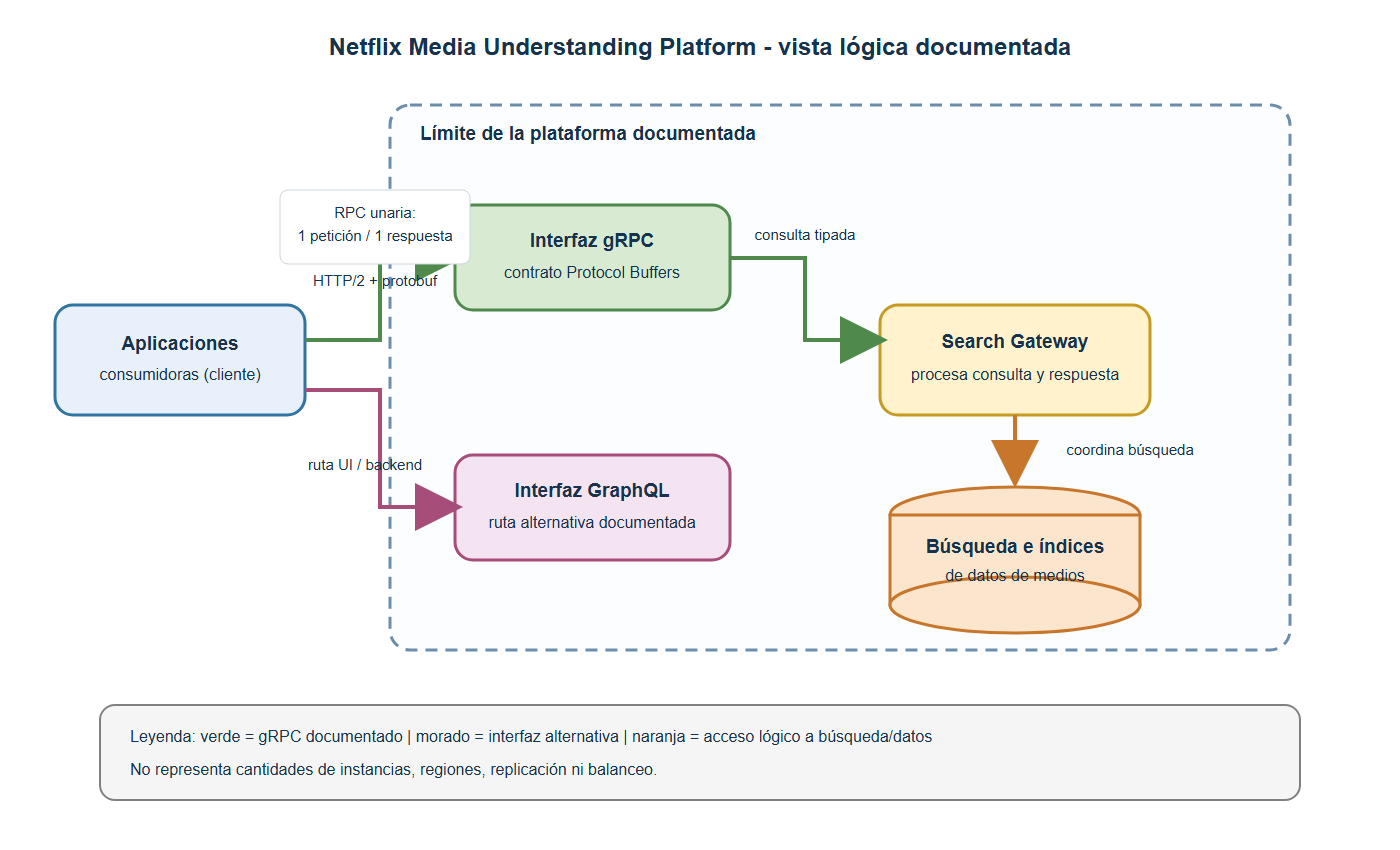
\includegraphics[width=0.96\linewidth]{figuras/arquitectura.png}
  \caption{Vista lógica original del caso documentado. Las flechas representan
  contratos de comunicación, no una topología física completa de Netflix.}
  \label{fig:arquitectura-steven}
\end{figure}

La aplicación consumidora actúa como cliente. Para una consulta, invoca un
método definido en un contrato Protocol Buffers mediante un \textit{stub}; la
infraestructura gRPC serializa la petición, la transporta por HTTP/2 y la
entrega al servicio. En el caso de una RPC unaria existe una petición y una
respuesta. El servicio que atiende la llamada cumple el rol de servidor, aunque
ese mismo proceso puede comportarse como cliente cuando consulta otro servicio.

En la plataforma documentada, el \textit{Search Gateway} concentra el
procesamiento de consultas y respuestas, y coordina el acceso a capacidades de
búsqueda e índices de datos de medios. La necesidad que resuelve gRPC no es
``hacer distribuido'' al sistema por sí solo: proporciona contratos tipados,
generación de clientes para distintos lenguajes y un mecanismo uniforme para
llamadas entre servicios. Esto reduce el trabajo de mantener bibliotecas de
cliente escritas manualmente y facilita la interoperabilidad del ecosistema de
microservicios.

La figura evita atribuir a gRPC funciones que pertenecen a otras capas. gRPC no
demuestra por sí mismo replicación, descubrimiento, balanceo, persistencia ni
tolerancia a fallos de Netflix. Esos mecanismos solo deben añadirse cuando una
fuente de Netflix los documente para el servicio analizado.

\paragraph{Fuentes técnicas.}
Netflix Technology Blog, ``Building a Media Understanding Platform for ML
Innovations'', 2023:
\url{https://netflixtechblog.com/building-a-media-understanding-platform-for-ml-innovations-9bef9962dcb7}.
Cloud Native Computing Foundation, ``How Netflix increased developer
productivity and defeated the thundering herd with gRPC'':
\url{https://www.cncf.io/case-studies/netflix/}.
Documentación oficial de gRPC, ``Core concepts, architecture and lifecycle'':
\url{https://grpc.io/docs/what-is-grpc/core-concepts/}.
